\subsection{Use Case Diagrams}
\begin{figure}[H]
	\begin{center}
		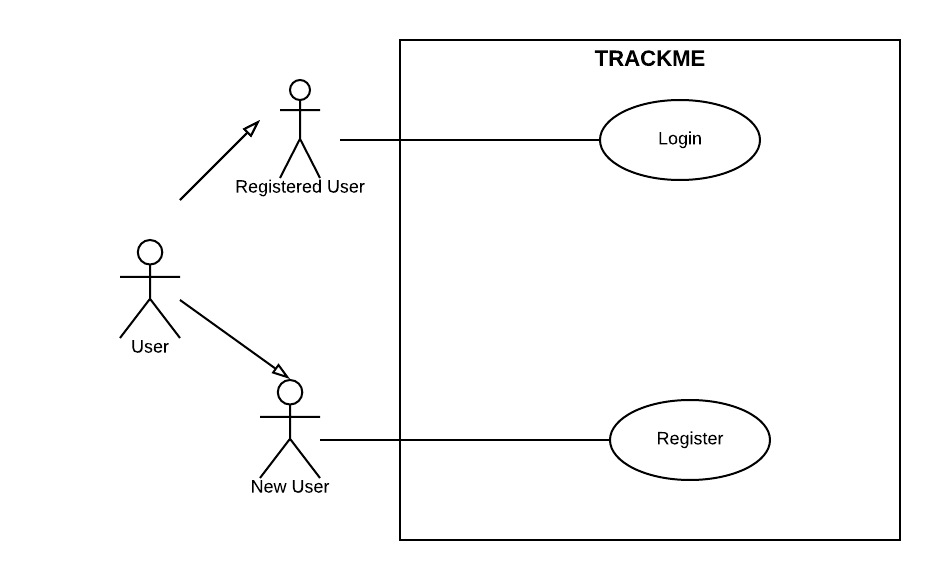
\includegraphics[width=\textwidth]{./RASD_Diagrams/UseCase_TrackMe.png}
      	\caption{Use case for TrackMe application}
        \label{TrackMe_usecase}
	\end{center}
\end{figure}


\begin{figure}[H]
	\begin{center}
		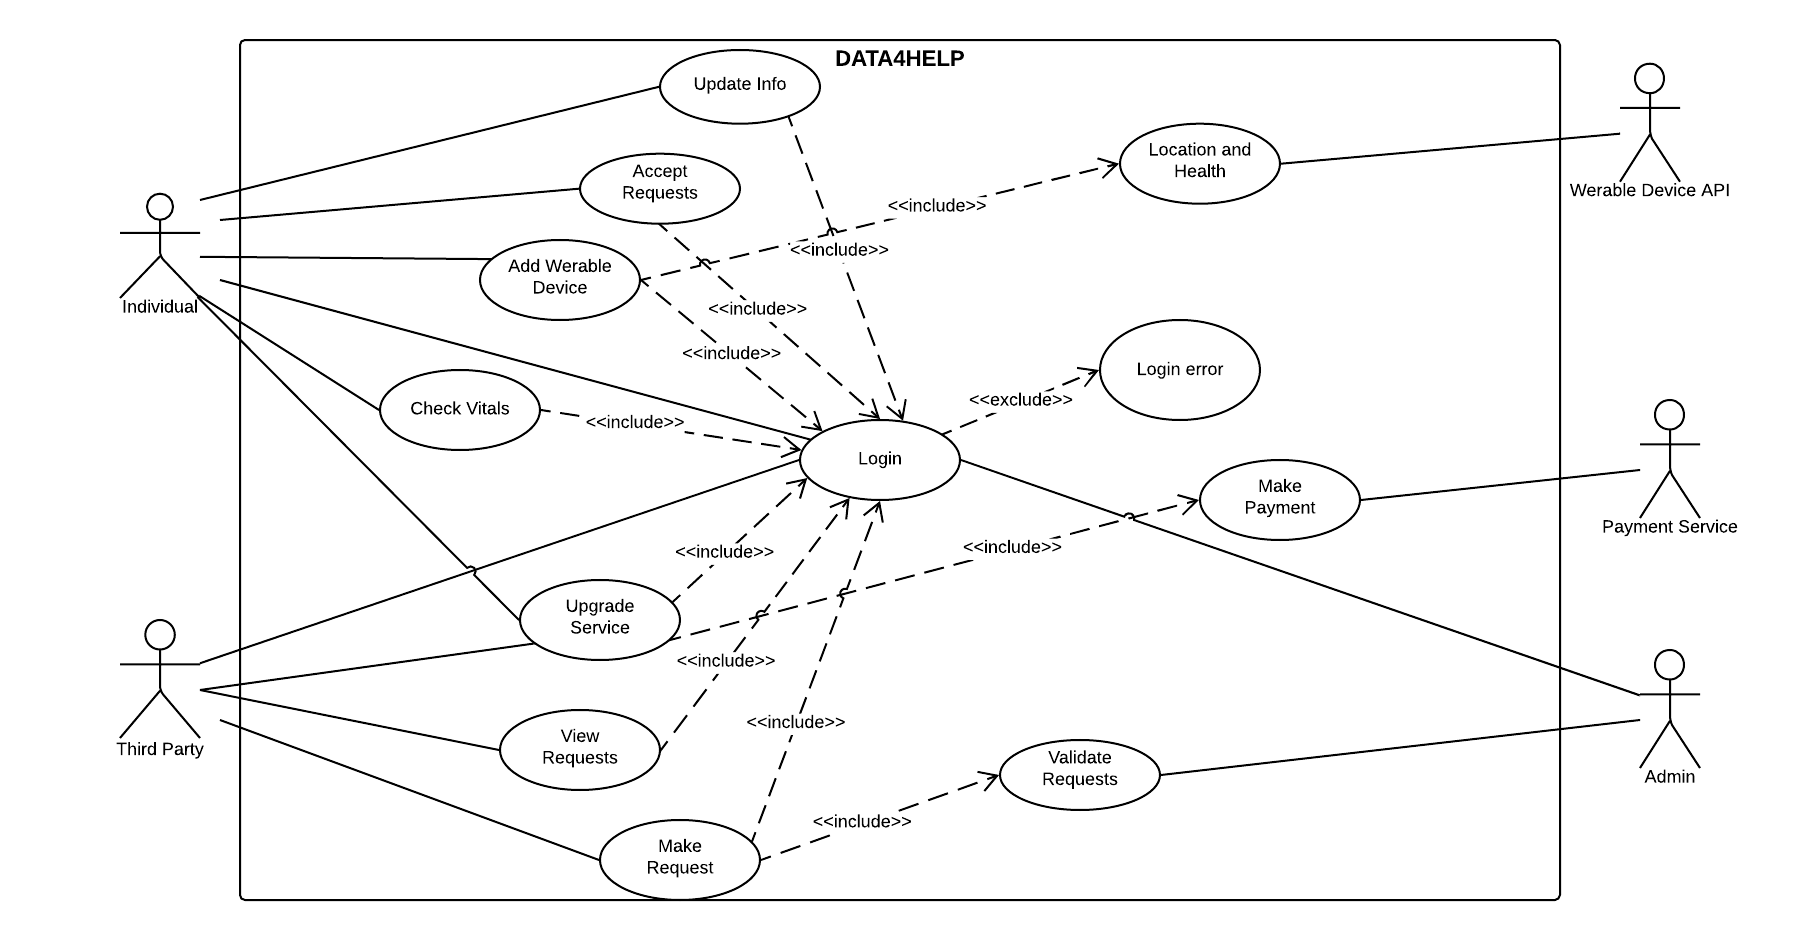
\includegraphics[width=\textwidth]{./RASD_Diagrams/UseCase_Data4Help.png}
        \caption{Use case for Data4help}
        \label{Data4help}
	\end{center}
\end{figure}

\begin{figure}[H]
	\begin{center}
		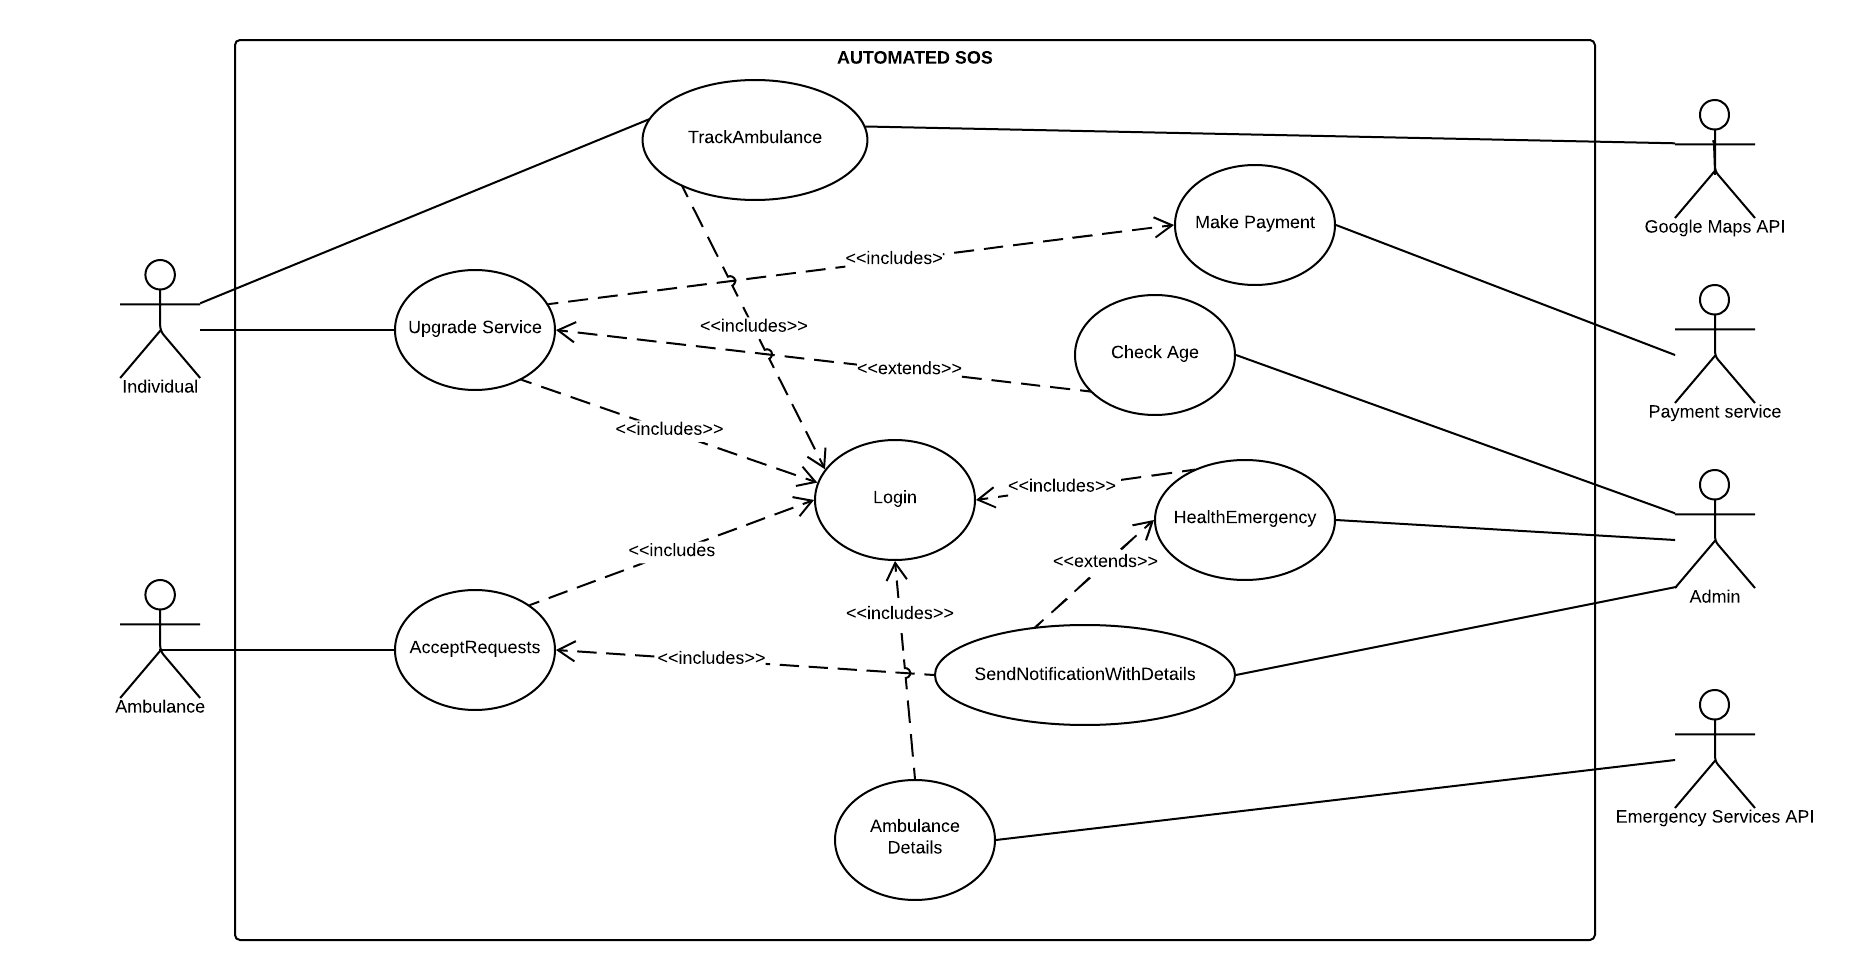
\includegraphics[width=\textwidth]{./RASD_Diagrams/UseCase_AutomatedSOS.png}
        \caption{Use case for Automated SOS}
        \label{track4run}
	\end{center}
\end{figure}

\begin{figure}[H]
	\begin{center}
		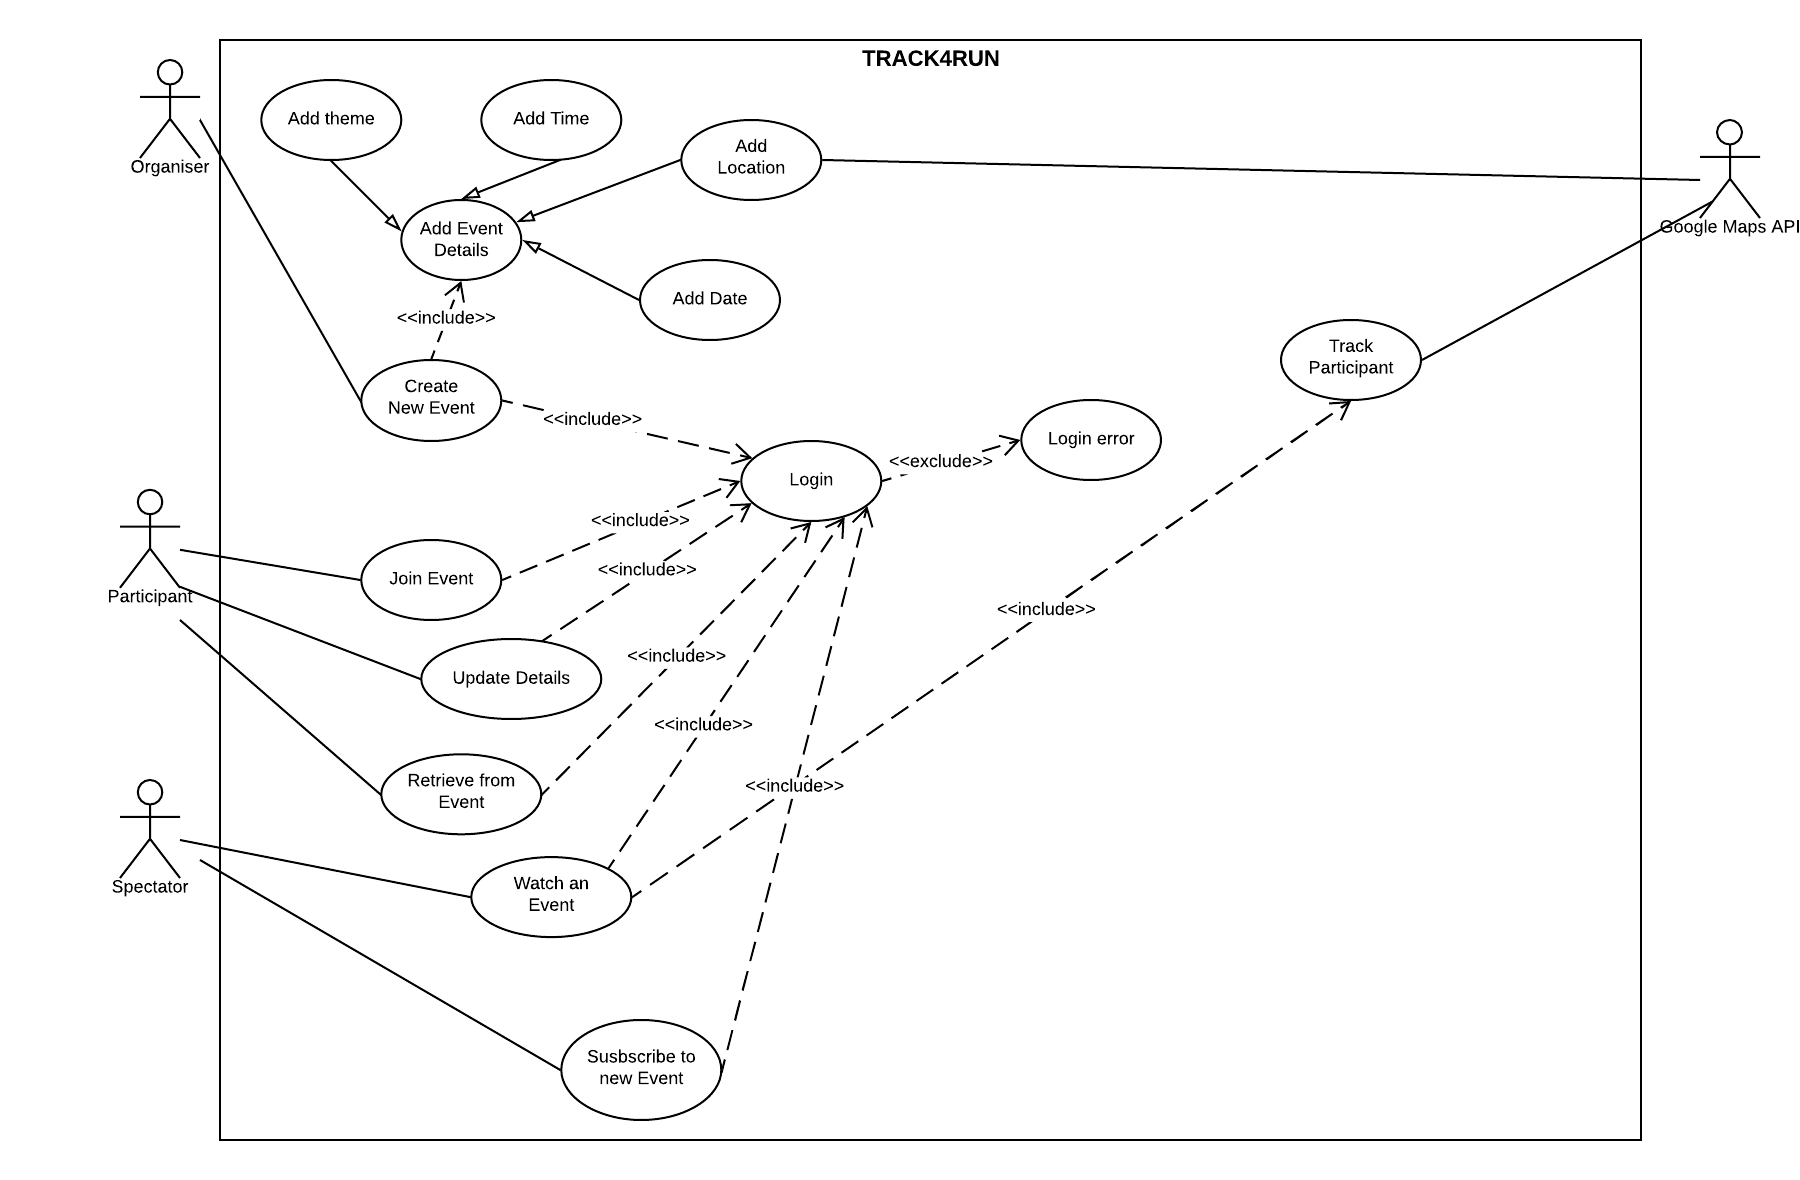
\includegraphics[width=\textwidth]{./RASD_Diagrams/UseCase_Track4Run.png}
        \caption{Use case for track4run}
        \label{track4run}
	\end{center}
\end{figure}


%================================Login===============================%
\begin{table}[H]
\begin{center}
\begin{tabular}{| l | p{0.75\textwidth} |}
\hline
Name & Login \\
\hline
Actors & Registered Users(Individual or Third Party)
\\
\hline
Entry condition & \begin{enumerate}
\item The user has successfully logged into the system
\item The user is not logged into the system yet
\end{enumerate}  \\
\hline
Event Flow & \begin{enumerate}
	\item The user opens the welcome page of the application and forwards to sign in
	\item He/She provides the valid credentials for login, say user name and password.
	\item User gets to authenticate into the application incase his credentials are valid.
    \item His/Her dashboard shows the services to which he/she is registered with.
	
\end{enumerate}
\\
\hline
Exit Conditions & The user successfully redirects to the dashboard. \\
\hline
Exception & 
The credentials provided by the user are invalid, in this case a login error message is shown and allows the user to input the username and password again.\\
\hline
\end{tabular}
\end{center}
\caption{Use case for Login.}
\label{usecase-login}
\end{table}

%========================Adding a Wearable device==========================%

\begin{table}[H]
\begin{tabular}{| l | p{0.75\textwidth} |}
\hline
Name & Add wearable Device\\
\hline
Actors & Individual\\
\hline
Entry condition & \begin{enumerate}
  \item The individual has successfully logged into the system.
  \item The individual has a wearable device supported by trackme
\end{enumerate}  \\
\hline
Event Flow & \begin{enumerate}
  \item Selects the add new wearable device button.
  \item Select the compatible device name from the given options.
  \item Connection successful.
\end{enumerate}
\\
\hline
Exit Conditions & The individual successfully connects to the device and navigates back to dashboard. \\
\hline
Exception & 
All devices are not compatible with TrackMe application. The user selects there wearable device among the list of compatible device from Dropdown. An error message is shown in case of connection problems.\\
\hline
\end{tabular}
\caption{Use case for adding a new wearable device.}
\label{usecase-adddevice}
\end{table}

%==========================Accept/Reject Requests=========================%


\begin{table}[H]
\begin{tabular}{| l | p{0.75\textwidth} |}
\hline
Name & Accept or Reject Requests\\
\hline
Actors & Individual\\
\hline
Entry condition & No entry conditions\\
\hline
Event Flow & \begin{enumerate}
\item The individual can see those requests made by a third party for specific individual health vitals or location.
\item He/She gets to accept or reject the requests.
\item The status of the request on the individual's dashboard will be updated with the corresponding response
\end{enumerate}
\\
\hline
Exit Conditions & The individual successfully redirects to the dashboard.\\
\hline
\end{tabular}
\caption{Use case for Accept or reject requests.}
\label{usecase-accorrejrequests}
\end{table}

%============================Update Info================================%
\begin{table}[H]
\begin{tabular}{| l | p{0.75\textwidth} |}
\hline
Name & Update Info\\
\hline
Actors & User\\
\hline
Entry condition & No entry conditions\\
\hline
Event Flow & \begin{enumerate}
\item Upon clicking on the update Info button, user gets to change the information given earlier.
\item Once he makes the corresponding changes, user can save it or cancel it.
\item Upon saving changes will be updated.
\end{enumerate}
\\
\hline
Exit Conditions & 
The user successfully redirects to the dashboard.\\
\hline
Exceptions & Upon providing invalid details, the user will be requested to enter the details again. Upon canceling the changes made would be lost.\\
\hline
\end{tabular}
\caption{Use case for Update Info requests.}
\label{usecase-taxiavailability}
\end{table}

%==========================Make Requests===============================================%
\begin{table}[H]
\begin{tabular}{| l | p{0.75\textwidth} |}
\hline
Name & Make Requests\\
\hline
Actors & Third Party\\
\hline
Entry condition & \begin{enumerate}
\item The third party is successfully logged into the system as a third party.
\item The third party needs needs health and location data of individuals or a group of individuals.
\end{enumerate}\\
\hline
Event Flow & \begin{enumerate}
\item The third party clicks the Make Requests button.
\item He/She/They are requested to select the type of request- individual or group of individuals.
\item Enter the valid reason for the request
\item Click the submit button.
\item The request is then validated by Trackme or individual according to the category.
\end{enumerate}
\\
\hline
Exit Conditions & The user successfully redirects to the dashboard once the requests is made.\\
\hline
\end{tabular}
\caption{Use case for Making requests.}
\label{usecase-Making-requests}
\end{table}

%====================================View Requests===================================%

\begin{table}[H]
\begin{tabular}{| l | p{0.75\textwidth} |}
\hline
Name & Check Status\\
\hline
Actors & Third Party\\
\hline
Entry condition & \begin{enumerate}
\item No entry conditions
\end{enumerate}\\
\hline
Event Flow & \begin{enumerate}
\item The Third Party clicks the Check status button.
\item The list of requests made by him/her is available with the status(approved or still waiting to be approved) of the requests
\end{enumerate}\\
\hline
Exit Conditions & The Third Party successfully navigates back.\\
\hline
Exceptions & Incase the Third Party has not made any requests a message stating “ No requests found” will be shown.\\
\hline
\end{tabular}
\caption{Use case for view requests.}
\label{usecase-view-requests}
\end{table}

%====================================Upgrade Service===================================%
\begin{table}[H]
\begin{tabular}{| l | p{0.75\textwidth} |}
\hline
Name & Upgrade Service\\
\hline
Actors & Third Party or Individual\\
\hline
Entry condition & The user needs to access a new service\\
\hline
Event Flow & \begin{enumerate}
\item The user clicks the service they want to upgrade.
\item Choose the duration for the service.
\item Directs to the payment page
\item Makes the payment and completes the transaction.
\end{enumerate}
\\
\hline
Exit Conditions & The user successfully redirects to the dashboard.\\
\hline
Exceptions & Transaction errors can happen, in that case he/she is asked to provide the credentials again and try. \\
\hline
\end{tabular}
\caption{Use case for Upgrade Service.}
\label{usecase-upgradeservice}
\end{table}

%==============================Validate Requests=======================================%

\begin{table}[H]
\begin{tabular}{| l | p{0.75\textwidth} |}
\hline
Name & Validate Requests\\
\hline
Actors & Admin\\
\hline
Assumptions & There are some requests made by the third party service.\\
\hline
Entry condition & No entry conditions\\
\hline
Event Flow & \begin{enumerate}
\item Checks for the latests requests and categorize them. 
\item Incase of requests for individuals the request is forwarded to the individual.
\item Incase of request for group of data, validity of reasons provided are checked. If the group of people requested for is greater than 1000, th request is accepted. 
\item Status of requests are updated.
\end{enumerate}
\\
\hline
Exit Conditions & None\\
\hline
Exceptions & If the requests are fake, then the requests are rejected. \\
\hline
\end{tabular}
\caption{Use case for Validate Requests.}
\label{usecase-validate-requests}
\end{table}
%==================================================================%
%               Automated SOS                                         %
%===================================================================%
%===================Send Notification to Ambulance Drivers=================================%
\begin{table}[H]
\begin{tabular}{| l | p{0.75\textwidth} |}
\hline
Name & Send Notification to Ambulance Drivers\\
\hline
Actors & Admin\\
\hline
Assumptions & The emergency health condition monitored is accurate as they are calculated on the basis of 3 readings.
\\
\hline
Entry condition & No entry conditions\\
\hline
Event Flow & \begin{enumerate}
\item Check for emergency condition of any individual.
\item Send push notification to all nearby ambulance drivers as soon as the emergency is encountered. The push notification guarantees a reaction time less than 5 seconds.
\item The push notification contains all the details of the individual.
\item The individual can also track the ambulance in their application's map.
\end{enumerate}
\\
\hline
Exit Conditions & None\\
\hline
Exceptions & None. \\
\hline
\end{tabular}
\caption{Use case for Send Push Notification.}
\label{usecase-push-notification}
\end{table}
%===================Accept individual request and navigate to their location=================================%
\begin{table}[H]
\begin{tabular}{| l | p{0.75\textwidth} |}
\hline
Name & Accept individual request and navigate to their location\\
\hline
Actors & Ambulance Driver\\
\hline
Assumptions &  The notification will be received by all nearby ambulance drivers and the first driver to accept the request will navigate to the individual's location.
\\
\hline
Entry condition & Receive a push notification and accept it.\\
\hline
Event Flow & \begin{enumerate}
\item The driver receives a push notification in the application for ambulance drivers.
\item They accept the request.
\item The first driver to accept the request navigates to individual's location with any emergency products if required.
\end{enumerate}
\\
\hline
Exit Conditions & Reject request\\
\hline
Exceptions & None. \\
\hline
\end{tabular}
\caption{Use case for Ambulance drivers accepting request.}
\label{usecase-ambulance-driver}
\end{table}
%==================================================================%
%               TRACK4RUN                                          %
%===================================================================%

%===================Create a New Event=================================%
\begin{table}[H]
\begin{tabular}{| l | p{0.75\textwidth} |}
\hline
Name & Create a new Event\\
\hline
Actors & Organizer\\
\hline
Assumptions & He/She needs to host a new event(race)\\
\hline
Entry condition & Must provide all event details and pay for organizing\\
\hline
Event Flow & \begin{enumerate}
\item Click on the create event Button
\item Enter the Details(Name, Location, Time, Reason)
\item Submit the details 
\end{enumerate}
\\
\hline
Exit Conditions & Event is successfully created and navigated to the dashboard\\
\hline
Exceptions & Incase the user gives an invalid location, he/she will be asked to re try again. Incase the location and time is already booked for another event a warning would be shown. \\
\hline
\end{tabular}
\caption{Use case for New Event/Race.}
\label{usecase-new-event/race}
\end{table}

%======================================Join Event=============================%

\begin{table}[H]
\begin{tabular}{| l | p{0.75\textwidth} |}
\hline
Name & Join Event\\
\hline
Actors & Participant\\
\hline
Assumptions & He/She needs to participate in an event\\
\hline
Entry condition & No entry conditions\\
\hline
Event Flow & \begin{enumerate}
\item He/She registers for an event 
\item Adds the required details which includes the wearable device,name, place etc.
\item Confirms the availability 
\item Submit the details
\end{enumerate}
\\
\hline
Exit Conditions & The Athlete successfully joins the event. \\
\hline
Exceptions & An error message would be generated incase the maximum limit for the participants have reached.\\
\hline
\end{tabular}
\caption{Use case for Joining an event/Race.}
\label{usecase-join-event/race}
\end{table}

%==================================Watch an event================================================%

\begin{table}[H]
\begin{tabular}{| l | p{0.75\textwidth} |}
\hline
Name & Watch an Event\\
\hline
Actors & Spectator\\
\hline
Entry condition & Should be logged in as a spectator\\
\hline
Event Flow & \begin{enumerate}
\item The user chooses the race which he wants to watch now.
\item Upon clicking a view, he/she can watch the race live.
\item He/She can navigate out whenever the user wants
\end{enumerate}
\\
\hline
Exit Conditions & Navigate back to the dashboard \\
\hline
Exceptions & Incase the user is not subscribed for any event, he/she won’t be able to see any. Incase the user has not made the payment, he/she won’t be able to watch the event. \\
\hline
\end{tabular}
\caption{Use case for watching an event/Race.}
\label{usecase-watch-event/race}
\end{table}


%+++++++++++++++++++++++++++++++++++++++++++++++++++++++++++++++++++++++++++++++++++++++++++++++++++++++%
%                                          SEQUENCE DIAGRAMS                                            %
%++++++++++++++++++++++++++++++++++++++++++++++++++++++++++++++++++++++++++++++++++++++++++++++++++++++++%
\subsection{Sequence Diagram}
1. Accept/Reject Third party requests:
\begin{figure}[H]
	\begin{center}
		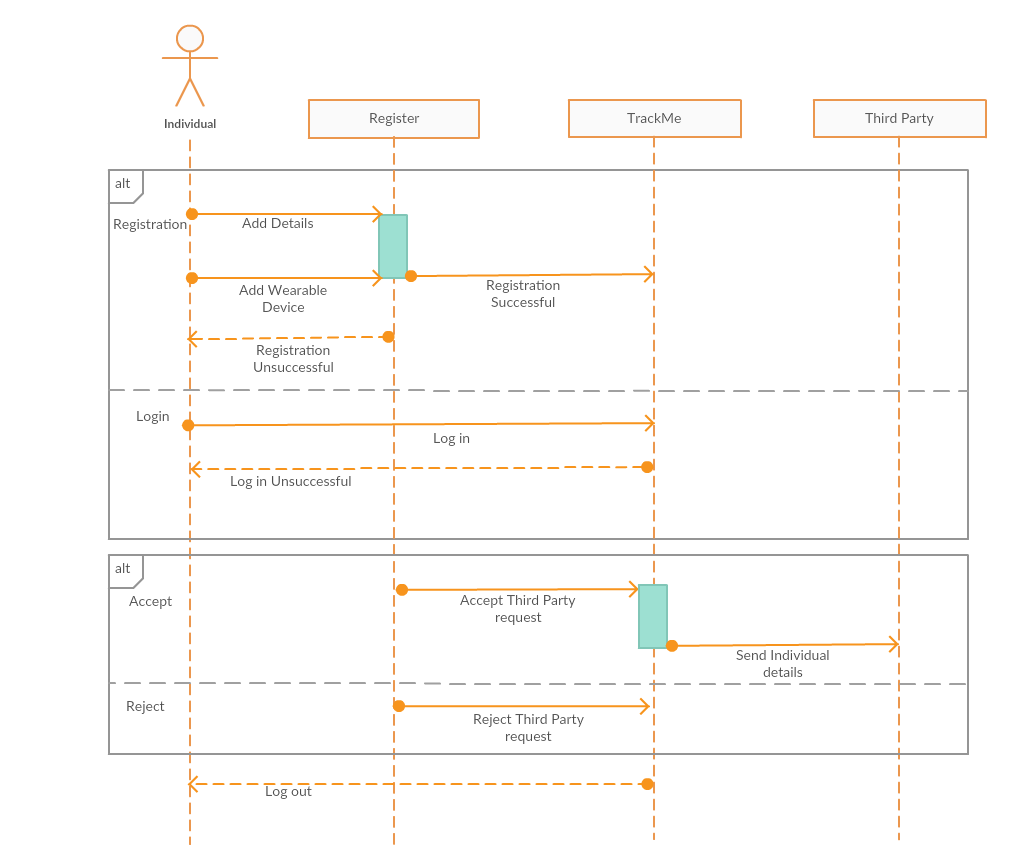
\includegraphics[width=\textwidth]{./RASD_Sequence/1__Individual.png}
      	\caption{Accept/Reject Third party requests.}
        \label{TrackMe_seq1}
	\end{center}
\end{figure}
.\newline\newline\newline\newline\newline\newline\newline\newline\newline\newline\newline
2. Third Party makes new request:
\begin{figure}[H]
	\begin{center}
		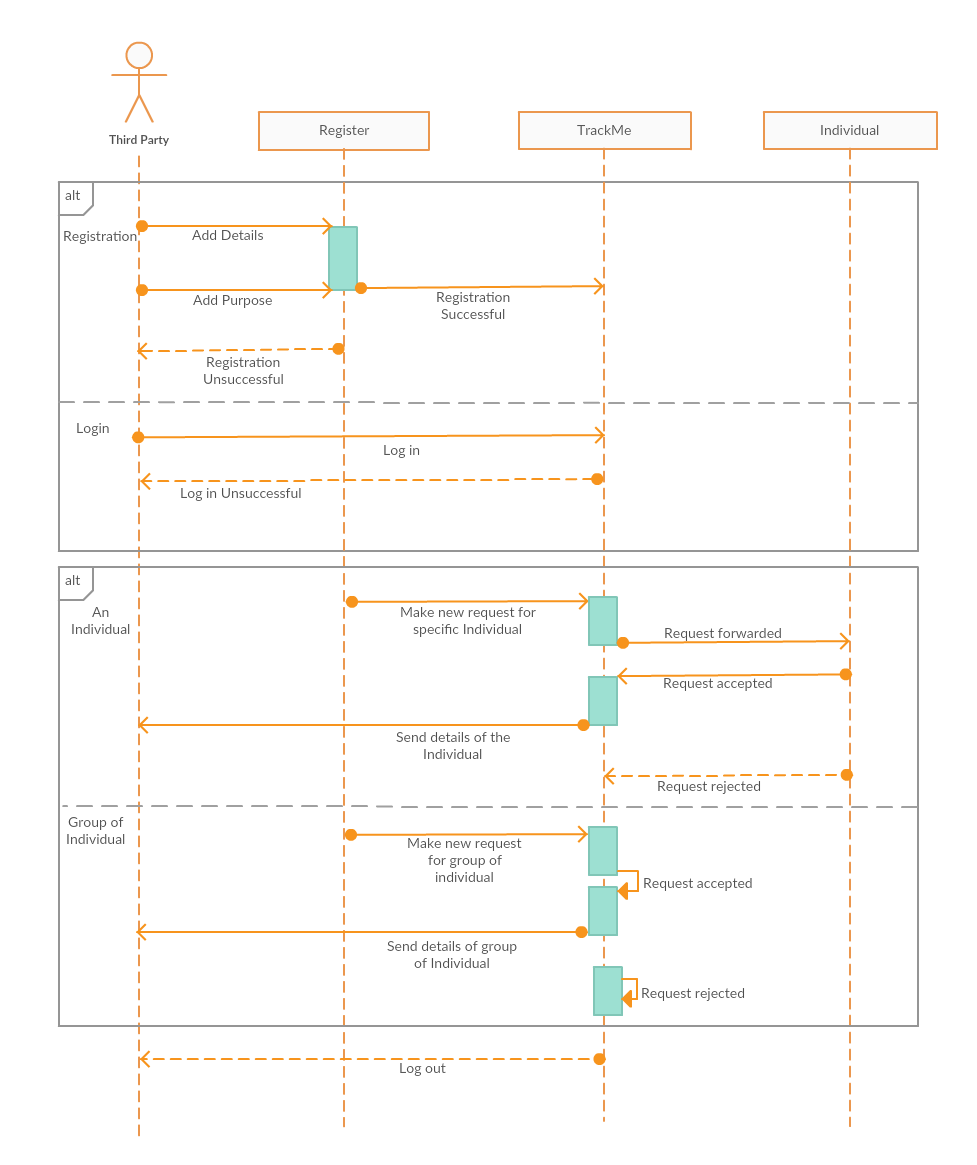
\includegraphics[width=\textwidth]{./RASD_Sequence/2__ThirdParty.png}
      	\caption{Third Party makes new request.}
        \label{TrackMe_seq2}
	\end{center}
\end{figure}
.\newline\newline
3. TrackMe validates request:
\begin{figure}[H]
	\begin{center}
		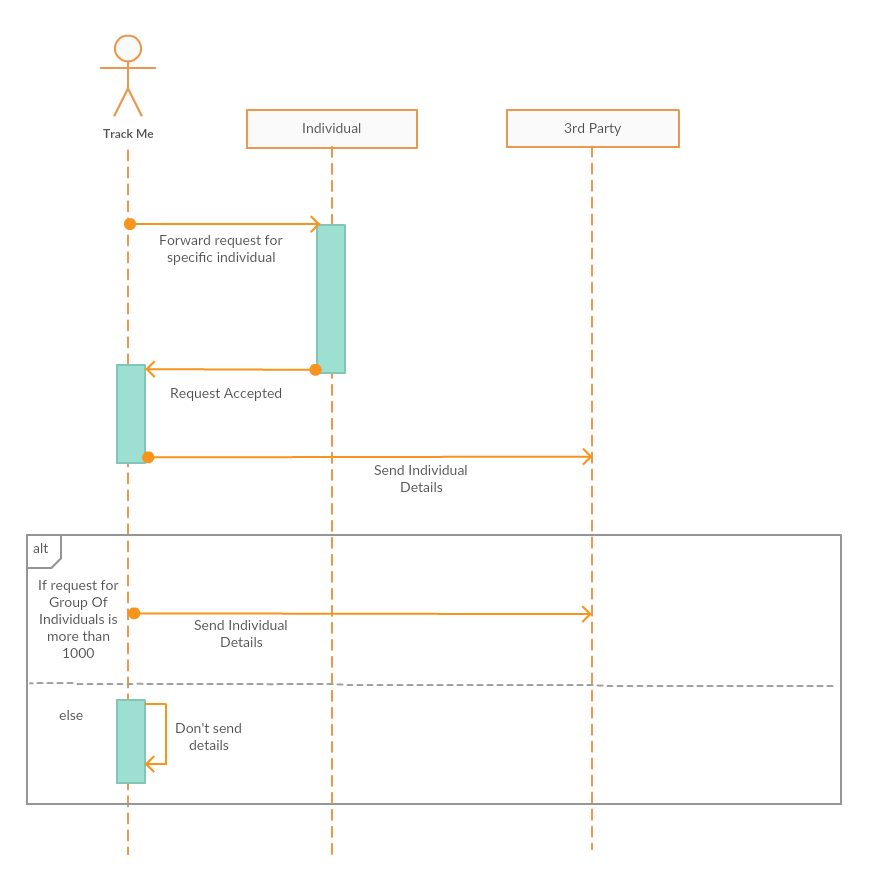
\includegraphics[width=\textwidth]{./RASD_Sequence/3__TrackMe.png}
      	\caption{TrackMe validates request.}
        \label{TrackMe_seq3}
	\end{center}
\end{figure}
.\newline\newline\newline\newline\newline\newline\newline\newline
4. Check vitals and send push notification:
\begin{figure}[H]
	\begin{center}
		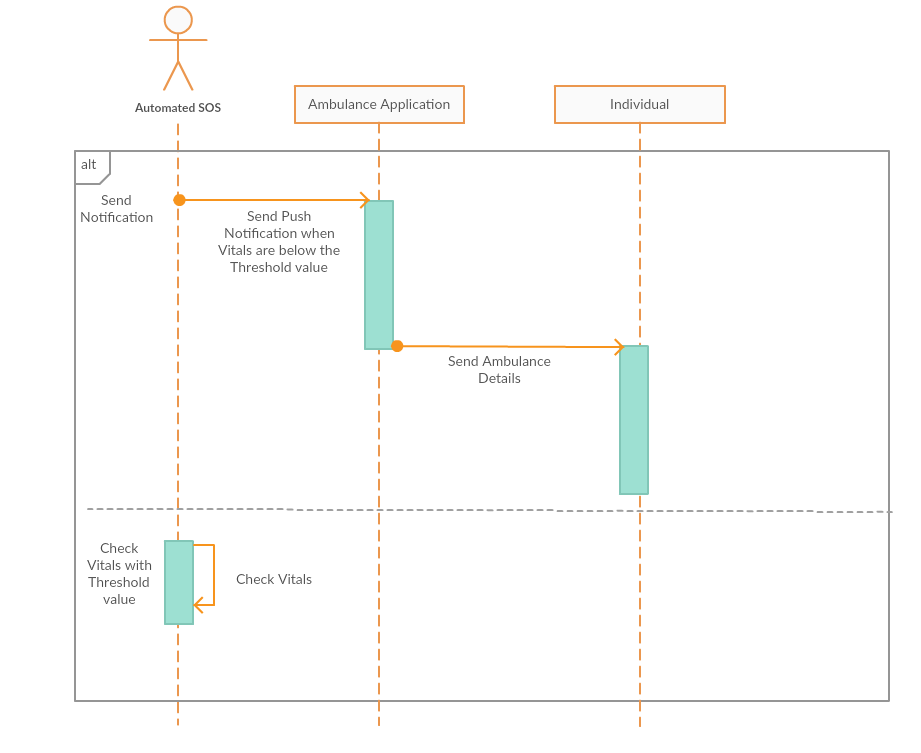
\includegraphics[width=\textwidth]{./RASD_Sequence/4_Automated_SOS.png}
      	\caption{Check vitals and send push notification.}
        \label{TrackMe_seq4}
	\end{center}
\end{figure}
.\newline\newline\newline\newline\newline\newline\newline\newline\newline\newline\newline\newline\newline
5. Ambulance Drivers accepts the request of push notifications and navigate to their location:
\begin{figure}[H]
	\begin{center}
		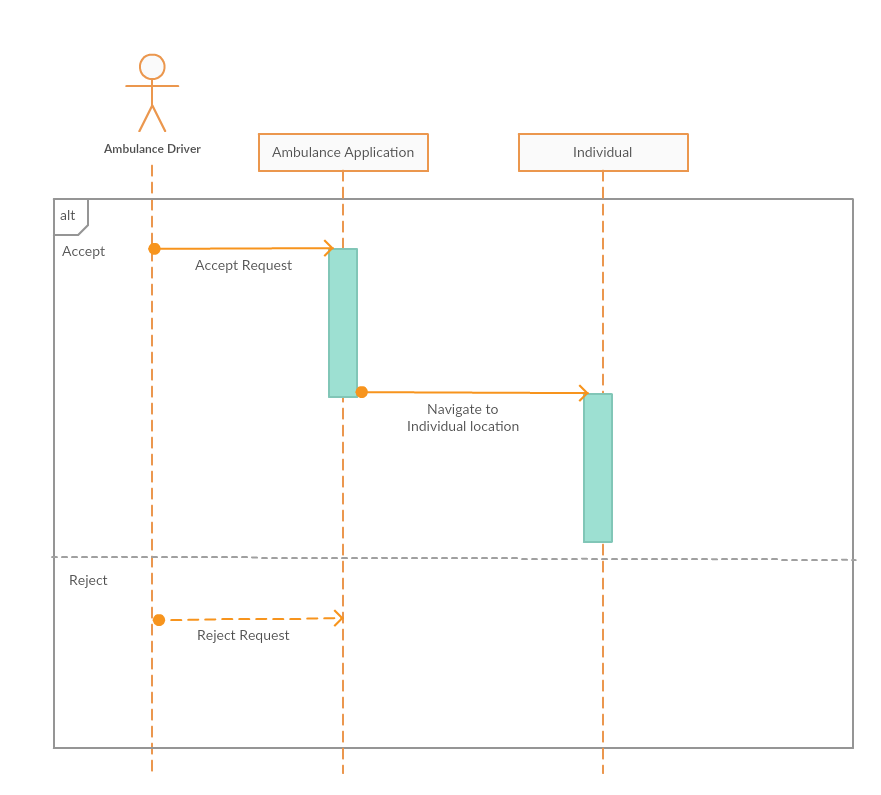
\includegraphics[width=\textwidth]{./RASD_Sequence/5_AmbulanceDriver.png}
      	\caption{Accept request of push notifications and Navigate to their location.}
        \label{TrackMe_seq5}
	\end{center}
\end{figure}
.\newline\newline\newline\newline\newline\newline\newline\newline\newline
6.Organizer adds race and defines path:
\begin{figure}[H]
	\begin{center}
		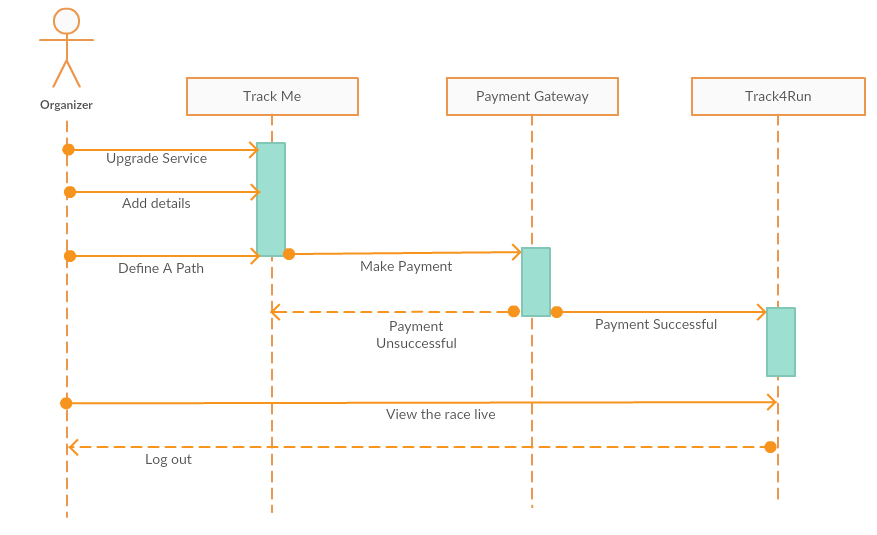
\includegraphics[width=\textwidth]{./RASD_Sequence/6_Organizer.png}
      	\caption{Organizer adds race and defines path.}
        \label{TrackMe_seq6}
	\end{center}
\end{figure}
.\newline\newline\newline\newline\newline\newline\newline\newline\newline\newline\newline\newline\newline\newline\newline\newline\newline\newline\newline
7. Athletes participate and Spectators view the race:
\begin{figure}[H]
	\begin{center}
		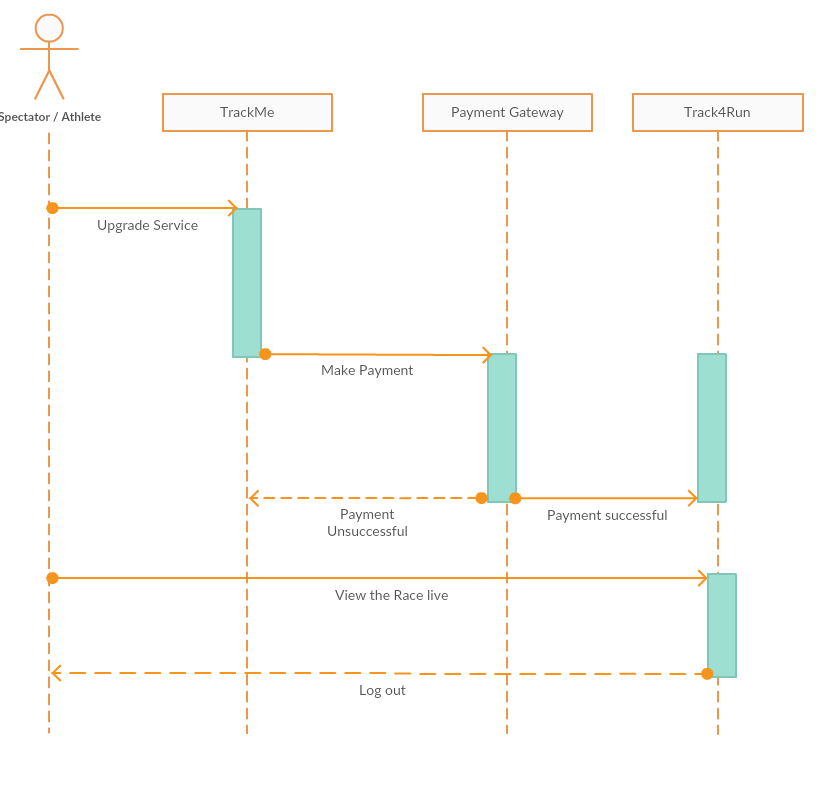
\includegraphics[width=\textwidth]{./RASD_Sequence/7_AthleteSpectator.png}
      	\caption{Athletes participate and Spectators view the race.}
        \label{TrackMe_seq7}
	\end{center}
\end{figure}
